\subsection{Benutzeroberfläche}

\sloppy
Die Benutzeroberfläche des RadarSimulators verwendet das Framework JavaFX und wird durch die \texttt{SimulatorMainContentProvider}-Klasse bereitgestellt. Der \texttt{SimulatorMainContentProvider} enthält verschiedene Einstellungsmöglichkeiten und stellt Klassen, welche die Funktionalität des   Benutzerinterface implementieren, zur Verfügung. Diese Klassen heißen FXML-Controller. Jeder FXML-Controller ist mit einer FXML-Datei verknüpft, welche die Anordnung der GUI-Komponenten auf zweidimensionaler Ebene definiert. 

Die Benutzeroberfläche besteht aus mehreren einzelnen Tabs. Dadurch werden die Funktionen des Simulators in unterschiedliche Bereiche eingeteilt. Jeder Tab hat einen Haupt FXML-Controller. Wenn der Controller einen zu großen Funktionsumfang hat, kann Funktionalität auf weitere FXML-Controller aufgeteilt werden. Der \texttt{SimulatorMainController} ist der oberste FXML-Controller. In ihm werden alle möglichen Tabs des Simulators vordefiniert und je nach Bedarf initialisiert. Welche Tabs geladen werden hängt davon ab, welcher Sensortyp und welche Asterix-Version ausgewählt ist. 

Zwischen Backend und Frontend gibt es keine definierte Schnittstelle. Die \texttt{Simulator\allowbreak Instance} wird beim Erzeugen des Controllers an das Frontend übergeben. Das heißt die FXML-Controller haben immer vollen Zugriff auf die \texttt{Simulatorinstance}. Das ist ein Problem, da Abhängigkeiten schnell unübersichtlich werden können und dadurch die Wartbarkeit des Systems erhöht wird.

Um das genauer zu erläutern wird das Beispiel aus dem Sequenzdiagramm \ref{img:AlterSimulator} genauer betrachtet. Auf der GUI-Oberfläche wird nun ein Bitfehler hinzugefügt. Daraufhin reagiert der entsprechende ActionListener. Er fügt den Bitfehler dem Model hinzu und sendet diesen über das Asterix-Interface an die Venus. Wenn die GUI Komponente das Model und den Sensor kontrolliert hat diese keine klare Aufgabe definiert. Bei einer modularen Architektur ist es bedeutsam, dass jede Komponente eine klar abgegrenzte Aufgabe \cite{modularSoftware} erfüllt. Somit ist diese Architektur fehlerhaft. Inwiefern die Funktion der View-Komponente verändert werden muss damit diese die Anforderungen einer modularen Architektur erfüllt wird in Kapitel XX geschildert.

\begin{figure}[h]
    \centering
    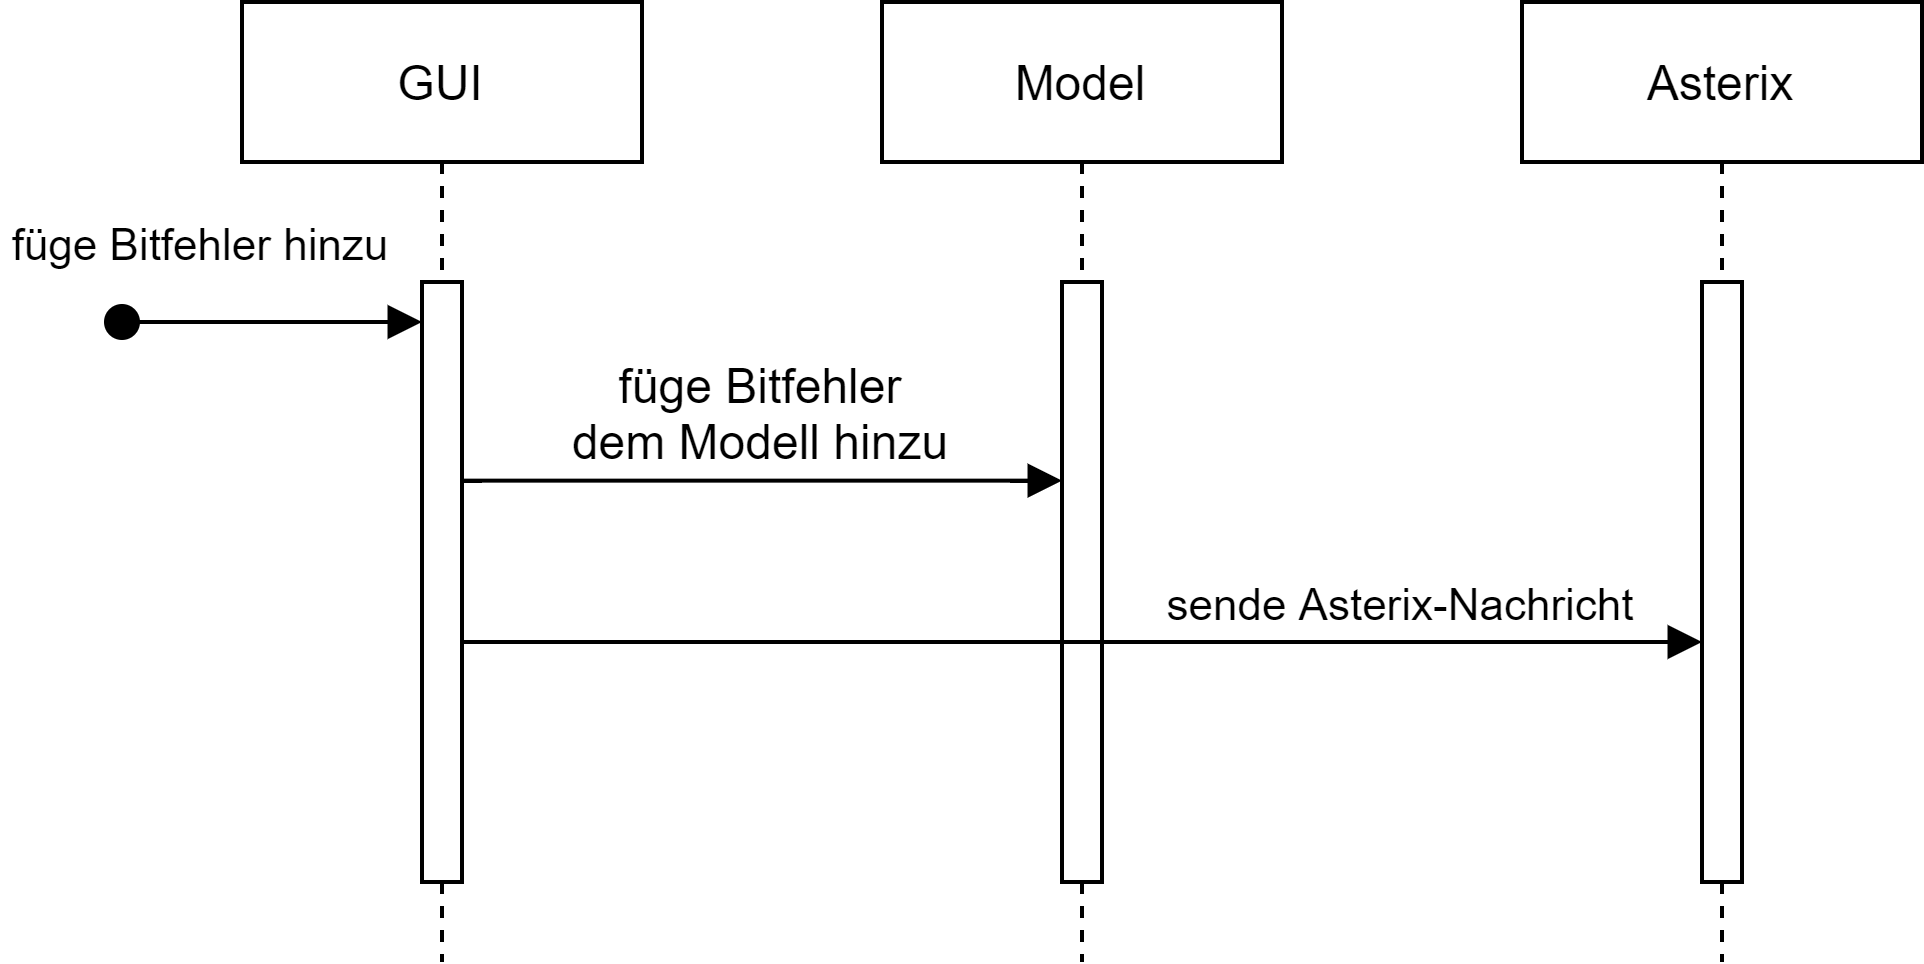
\includegraphics[width=0.8\textwidth]{content/assets/Kapitel3/AlterSimulator.png}
    \caption{UI - Alter Simulator}
    \label{img:AlterSimulator}
\end{figure}

Weitere Optimierung bedarf es bei der Initialisierung der Tabs. Die späteren Anwendungen haben unterschiedlich viele Tabs. Die genaue Übersicht gibt es 
in \ref{fig:TabsPerApp}

\begin{figure}[ht]
    \centering
    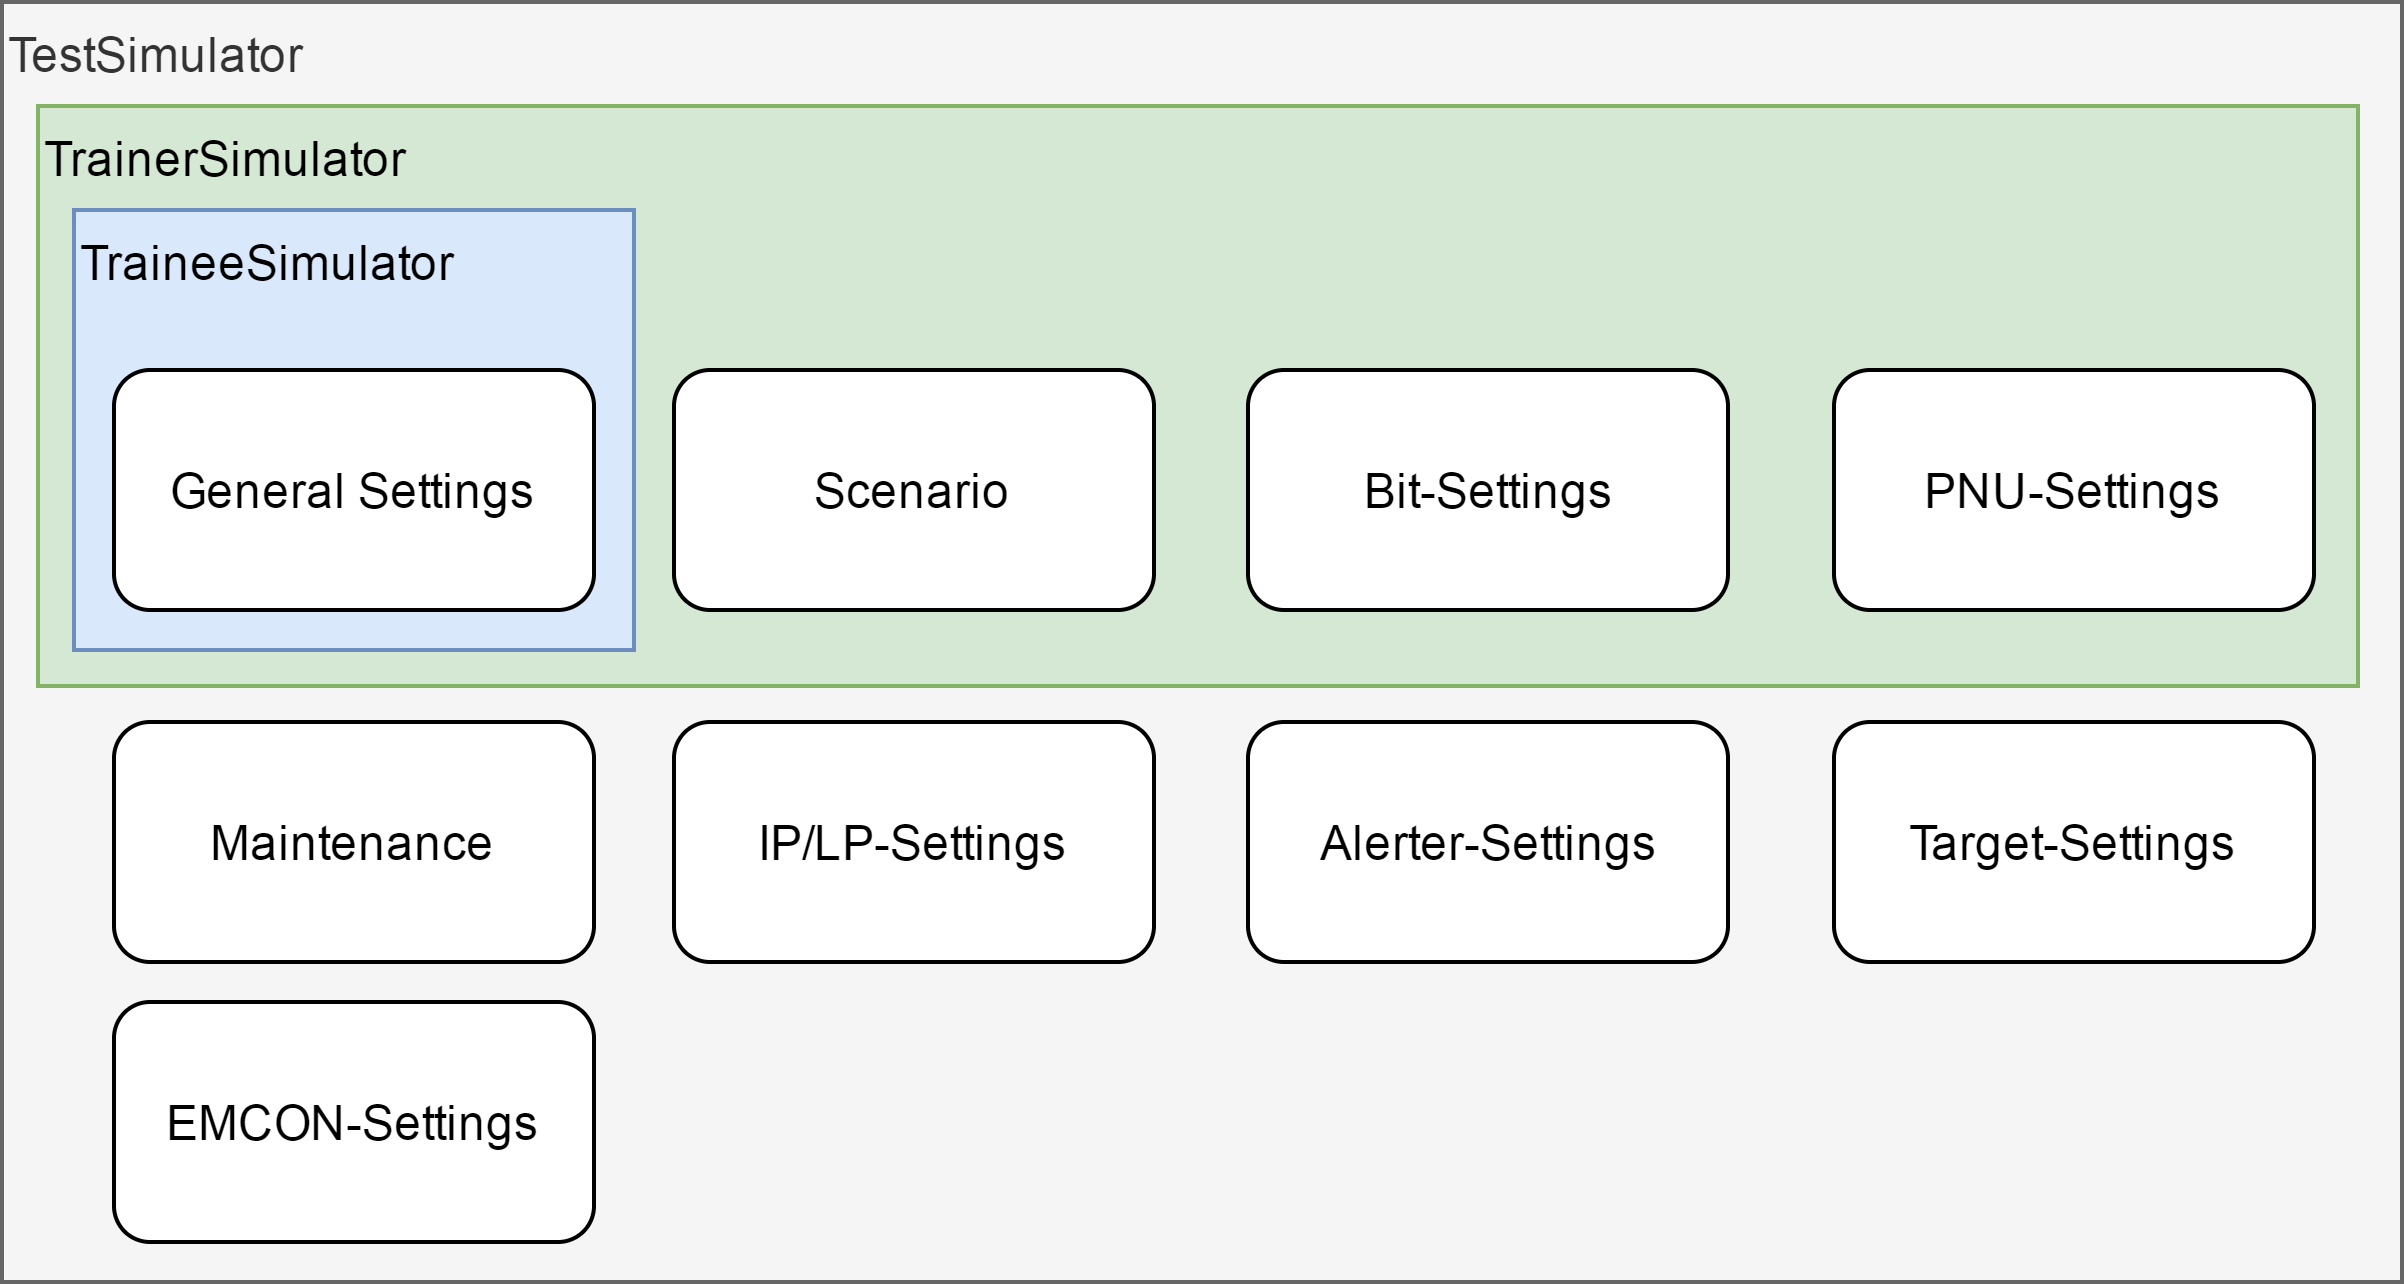
\includegraphics[width=0.8\textwidth]{content/assets/Kapitel3/TabsPerApp.png}
    \caption{UI - Alter Simulator}
    \label{fig:TabsPerApp}
\end{figure}

Deshalb ist es entweder notwendig für jede Anwendung einen separaten SimulatorMainController zu konfigurieren. Daraus würde redundanter Code entstehen, 
den man so gut es geht, vermeiden möchte. Die Alternative wäre eine allgemeinen SimulatorMainController, welcher alle verfügbaren Tabs im OSGi-Kontext 
lädt. Um das zu implementieren können Extension Points verwendet werden.
